\documentclass[
11pt, % The default document font size, options: 10pt, 11pt, 12pt
codirector, % Uncomment to add a codirector to the title page
]{charter} 




% El títulos de la memoria, se usa en la carátula y se puede usar el cualquier lugar del documento con el comando \ttitle
\titulo{Red de sensores para monitoreo ambiental en laboratorios críticos} 

% Nombre del posgrado, se usa en la carátula y se puede usar el cualquier lugar del documento con el comando \degreename
%\posgrado{Carrera de Especialización en Sistemas Embebidos} 
\posgrado{Carrera de Especialización en Internet de las Cosas} 
%\posgrado{Carrera de Especialización en Intelegencia Artificial}
%\posgrado{Maestría en Sistemas Embebidos} 
%\posgrado{Maestría en Internet de las cosas}

% Tu nombre, se puede usar el cualquier lugar del documento con el comando \authorname
\autor{Ing. Christian Canaan Castro Botek} 

% El nombre del director y co-director, se puede usar el cualquier lugar del documento con el comando \supname y \cosupname y \pertesupname y \pertecosupname
%\director{Nombre del Director}
\pertenenciaDirector{Esp. Ing. Pedro Rosito} 
% FIXME:NO IMPLEMENTADO EL CODIRECTOR ni su pertenencia
%\codirector{John Doe} % para que aparezca en la portada se debe descomentar la opción codirector en el documentclass
\pertenenciaCoDirector{FIUBA}

% Nombre del cliente, quien va a aprobar los resultados del proyecto, se puede usar con el comando \clientename y \empclientename
\cliente{Ing. Guillermo Kirsch}
\empresaCliente{FLEXAR S.R.L.}

% Nombre y pertenencia de los jurados, se pueden usar el cualquier lugar del documento con el comando \jurunoname, \jurdosname y \jurtresname y \perteunoname, \pertedosname y \pertetresname.
\juradoUno{Nombre y Apellido (1)}
\pertenenciaJurUno{pertenencia (1)} 
\juradoDos{Nombre y Apellido (2)}
\pertenenciaJurDos{pertenencia (2)}
\juradoTres{Nombre y Apellido (3)}
\pertenenciaJurTres{pertenencia (3)}
 
\fechaINICIO{28 de febrero de 2023}		%Fecha de inicio de la cursada de GdP \fechaInicioName
\fechaFINALPlan{11 de abril de 2023} 	%Fecha de final de cursada de GdP
\fechaFINALTrabajo{25 de agosto de 2023}	%Fecha de defensa pública del trabajo final


\begin{document}

\maketitle
\thispagestyle{empty}
\pagebreak


\thispagestyle{empty}
{\setlength{\parskip}{0pt}
\tableofcontents{}
}
\pagebreak


\section*{Registros de cambios}
\label{sec:registro}


\begin{table}[ht]
\label{tab:registro}
\centering
\begin{tabularx}{\linewidth}{@{}|c|X|c|@{}}
\hline
\rowcolor[HTML]{C0C0C0} 
Revisión & \multicolumn{1}{c|}{\cellcolor[HTML]{C0C0C0}Detalles de los cambios realizados} & Fecha      \\ \hline
1      & Creación del documento                                 &\fechaInicioName \\ \hline
2      & Se aplicaron correcciones y se completa hasta el punto 9 inclusive. & 21 de marzo de 2023 \\ \hline
3      & Se aplicaron correcciones y se completa hasta el punto 12 inclusive. & 26 de marzo de 2023 \\ \hline
\end{tabularx}
\end{table}

\pagebreak



\section*{Acta de constitución del proyecto}
\label{sec:acta}

\begin{flushright}
Buenos Aires, \fechaInicioName
\end{flushright}

\vspace{2cm}

Por medio de la presente se acuerda con el \authorname\hspace{1px} que su Trabajo Final de la \degreename\hspace{1px} se titulará ``\ttitle'', consistirá esencialmente en la implementación de un prototipo de un sistema de monitoreo ambiental para laboratorios críticos, y tendrá un presupuesto preliminar estimado de 600 h de trabajo y \textcolor{red}{\$XXX}, con fecha de inicio \fechaInicioName\hspace{1px} y fecha de presentación pública \fechaFinalName.

Se adjunta a esta acta la planificación inicial.

\vfill

% Esta parte se construye sola con la información que hayan cargado en el preámbulo del documento y no debe modificarla
\begin{table}[ht]
\centering
\begin{tabular}{ccc}
\begin{tabular}[c]{@{}c@{}}Dr. Ing. Ariel Lutenberg \\ Director posgrado FIUBA\end{tabular} & \hspace{2cm} & \begin{tabular}[c]{@{}c@{}}\clientename \\ \empclientename \end{tabular} \vspace{2.5cm} \\ 
\multicolumn{3}{c}{\begin{tabular}[c]{@{}c@{}} \supname \\ Director del Trabajo Final\end{tabular}} \vspace{2.5cm} \\
%\begin{tabular}[c]{@{}c@{}}\jurunoname \\ Jurado del Trabajo Final\end{tabular}     &  & \begin{tabular}[c]{@{}c@{}}\jurdosname\\ Jurado del Trabajo Final\end{tabular}  \vspace{2.5cm}  \\
%\multicolumn{3}{c}{\begin{tabular}[c]{@{}c@{}} \jurtresname\\ Jurado del Trabajo Final\end{tabular}} \vspace{.5cm}                                                                     
\end{tabular}
\end{table}




\section{1. Descripción técnica-conceptual del proyecto a realizar}
\label{sec:descripcion}

En FLEXAR S.R.L. se fabrican celdas de carga (figura 1) para todo tipo de aplicaciones tales como pesaje de vehículos, pesajes de movimiento, balanzas de piso, tanques, tolvas, etc. El proceso productivo de las celdas precisan el monitoreo y cuidado de cuatro plantas separadas pero próximas entre sí, todas ubicadas en la zona urbano-industrial de la localidad de San Martín, Buenos Aires, Argentina. En tres de las planta, se realizan diversas tareas que pretenden cierto grado de exigencia y calidad que pueden verse afectadas ante cualquier perturbación externa o factor medio ambiental. Estos procesos son tan críticos que de no cumplir con los estándares internacionales, nacionales y empresariales conllevan a grandes perdidas para la empresa, tanto económicas como de confianza mercantil. 

Es por ello que bajo este contexto se busca implementar un sistema automático, de bajo costo y mantenimiento que permita implementar una red de sensores para el monitoreo y control ambiental de dichos laboratorios. Como requisito primario, la red de sensores debe estar basada en la familia de chips SoC (System-on-a-Chip) de bajo coste y consumo de energía ESP32, sensores DHT22, alimentación provista por la red, conectividad Wi-Fi y una web de tipo SPA desarrollada con el framework de VueJS para la visualización y monitoreo de las variables de interés. En la figura 2 se puede observar la composición básica del sistema.

\begin{figure}[h!]
\centering 
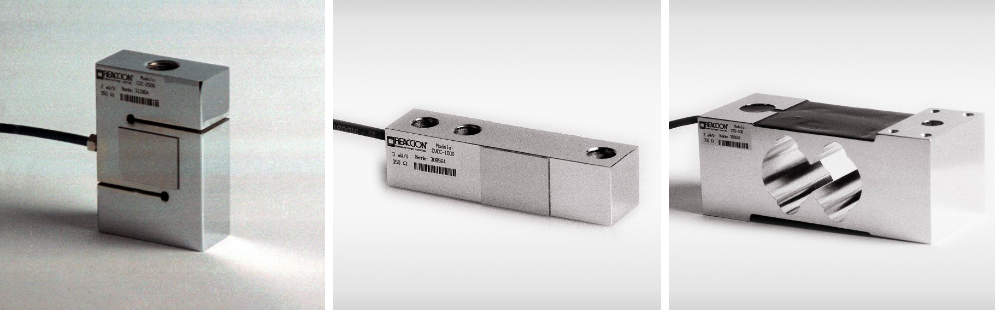
\includegraphics[width=.8\textwidth]{./Figuras/Celdas.png}
\caption{Distintos modelos de celdas.}
\label{fig:descripcion}
\end{figure}

\begin{figure}[h!]
\centering 
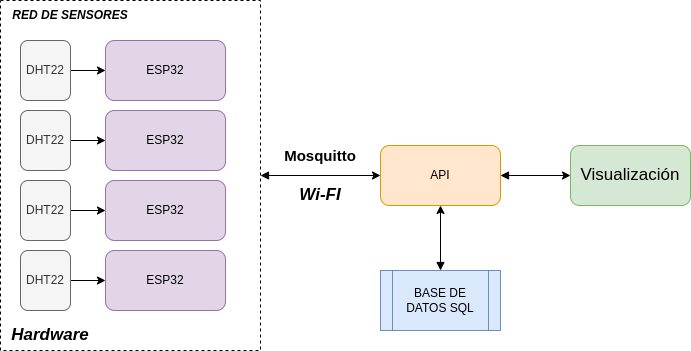
\includegraphics[width=.8\textwidth]{./Figuras/CompoBasica.png}
\caption{Composición básica del sistema.}
\label{fig:descripcion}
\end{figure}

\section{2. Identificación y análisis de los interesados}
\label{sec:interesados}

Cliente: Ing. Guillermo Kirsch tiene amplios y diversos conocimientos técnicos y es un gran guía para la elaboración del proyecto pero no dispone de mucho tiempo por tener una gran responsabilidad laboral en otras áreas de la empresa. Sin embargo, estará presente en gran parte del desarrollo, testeo y puesta en marcha de este proyecto. 

Colaborador: Ing. Luciano Rossi es el responsable de guiar supervisar y guiar al equipo de desarrollo de software de la empresa, estará presente en gran parte del desarrollo y testeo de este proyecto.

\begin{table}[h]
%\caption{Identificación de los interesados}
%\label{tab:interesados}
\begin{tabularx}{\linewidth}{@{}|l|X|X|l|@{}}
\hline
\rowcolor[HTML]{C0C0C0} 
Rol           & Nombre y Apellido & Organización 	& Puesto 	\\ \hline
%Auspiciante   &                   &              	&        	\\ \hline
Cliente       & \clientename      &\empclientename	& Gerente de Ingeniería       	\\ \hline
%Impulsor      &                   &              	&        	\\ \hline
Responsable   & \authorname       & FIUBA        	& Alumno 	\\ \hline
Colaboradores & Luciano Rossi                & FLEXAR S.R.L           	& Desarrollo de software       	\\ \hline
Orientador    & \pertesupname	      & FIUBA 	& Director	Trabajo final \\ \hline
%Equipo        & miembro1 \newline 
%				miembro2          &              	&        	\\ \hline
%Opositores    &                   &              	&        	\\ \hline
Usuario final & \clientename                 & FLEXAR S.R.L             	&  Gerente de Ingeniería      	\\ \hline
\end{tabularx}
\end{table}

\section{3. Propósito del proyecto}
\label{sec:proposito}

El propósito de este proyecto es poder diseñar e implementar el prototipo de una red de sensores para el monitoreo y control de variables de temperatura y humedad sobre los distintos laboratorios de tareas críticas de la empresa FLEXAR S.R.L. lo que permitirá adjuntar a las especificaciones de cada celda información adicional respecto a las condiciones ambientales a las que se encontraron expuestas durante el proceso productivo. Adicionalmente, también facilitará detectar causas de fallas en lotes de producción.

\section{4. Alcance del proyecto}
\label{sec:alcance}

El presente proyecto incluye la elaboración del prototipo de red basada en ESP32 que reporte, almacene y permita la visualización a través de una web las variables medidas para cada laboratorio de interés.

Se incluye:
\begin{itemize}
\item El armado de al menos dos prototipos de nodos de medición con ESP32.
\item Elaboración de la red de comunicación de estos dispositivos con la base de datos de la empresa.
\item Implementación de una estrategia de comunicación de datos segura.
\item Desarrollo de un front-end.
\item Muestra y visualización de los datos en tiempo real.
\item Documentación sobre el proyecto.
\end{itemize}

No se incluye:
\begin{itemize}
\item Análisis de trafico de datos.
\item Implementación de testing sobre el software desarrollado.
\item Implementación de una estrategia de comunicación de datos segura.
\item Visualización estadística de los datos.
\item Compatibilidad con dispositivos móviles.
\end{itemize}


\section{5. Supuestos del proyecto}
\label{sec:supuestos}

Para el cumplimiento de este proyecto se supone que: 

\begin{itemize}
\item Se dispondrá del tiempo y espacio para realizar distintas pruebas.
\item Habrá recursos económicos para la construcción del hardware.
\item Los tiempos fabricación estarán dentro de los márgenes habituales.
\item Existirá comunicación permanente con el cliente para solventar dudas.
\item Los tiempos de autonomía del hardware estarán basados en cálculos pesimistas y no en ensayos controlados.
\item Se tendrá acceso a todos los recursos digitales de la empresa tales como acceso a las bases de datos, red, etc. para agregar el sistema desarrollado en este trabajo a los demás sistemas de la empresa.
\end{itemize}


\section{6. Requerimientos}
\label{sec:requerimientos}

Los requerimientos del proyecto fueron convenidos por ambas partes a través del documento inicial de presentación del proyecto y distintas reuniones coordinadas. 

\begin{enumerate}
	\item Requerimientos generales del proyecto:
	\begin{enumerate}
	\item Deadline 1 Diciembre 2023.
	\item Entregable prototipo de hardware funcional y prototipo de aplicación con función de visualización de los datos en tiempo real de agrupados por sector.
	\end{enumerate}
\item Requerimientos físicos del sistema:
	\begin{enumerate}
	\item Prototipo del hardware basado en ESP32 y DHT22.
	\item Alimentación desde la red.
	\item Resistente a condiciones ambientales, con grado de protección IP60.
	\end{enumerate}
\item Requerimientos funcionales del sistema:
	\begin{enumerate}
	\item Hardware:
		\begin{enumerate}
		\item Contará con pines de acceso para el cargado de firmware.
		\item Envío de datos por MQTT.
		\item No enfocarse en el consumo por estar conectado a la red.
		\item Uso eficiente de la red de comunicación.
		\item Baja tasa de transferencia de datos.
		\item Bajo costo, siempre se busca ahorrar.
		\end{enumerate}
	\item Software y aplicación:
		\begin{enumerate}
		\item Almacenamiento de la información en base de datos postgressql.
		\item Validación de usuario para el ingreso a la plataforma.
		\item Capacidad de escalabilidad para registrar nuevos nodos de medición.
		\item Grafica histórica de los niveles de temperatura y humedad.
		\item Visualización de datos en tiempo real.
		\item Bajo tráfico de datos.
		\item Comunicación segura.
		\item Sistema de alarma en caso de una medición fuera de rango aceptable.
		\end{enumerate}
	\end{enumerate}
\item Requerimientos de documentación:
	\begin{enumerate}
	\item Elaboración de un informe de avance del proyecto.
	\item Elaboración de informe de puesta en marcha.
	\item Documentación general del desarrollo del software y estructura de la base de datos.
	\item Memoria de trabajo final.
	\end{enumerate}	
\end{enumerate}


\section{7. Historias de usuarios (\textit{Product backlog})}
\label{sec:backlog}

Ponderación: según el esfuerzo que requiera el cumplimiento de la historia.

Prioridad: de 1 al 10 considerando 10 como lo más importante.

Se define como usuario aquel quien hace un uso general del sistema.

Calificación: Ponderación - Prioridad.

\begin{itemize}
\item Como gerente de FLEXAR S.R.L. quiero una aplicación que me permita visualizar datos ambientales en tiempo real. \textit{10-10}
\item Como gerente de FLEXAR S.R.L. quiero un dispositivo que permita visualizar datos historicos ambientales \textit{8-10}
\item Como gerente de FLEXAR S.R.L. quiero que el dispositivo sea compatible con la infraestructura ya existente para mayor interoperabilidad y soporte. \textit{9-10}
\item Como gerente de FLEXAR S.R.L. quiero que la información sea visible en una web responsiva para tener mayor portabilidad. \textit{10-10}
\item Como gerente de FLEXAR S.R.L. quiero una interfaz gráfica para tener un login de usuario. \textit{7-10}
\item Como usuario operario quiero una aplicación para que funcione en un smartphone. \textit{5-7}
\item Como usuario operario quiero una aplicación de fácil acceso. \textit{7-7}
\item Como gerente de FLEXAR S.R.L. quiero que el dispositivo funcione el mayor tiempo posible para facilitar la instalación y el mantenimiento. \textit{8-10}
\item Como gerente de FLEXAR S.R.L. quiero un sistema escalable. \textit{10-10}
\item Como gerente de FLEXAR S.R.L. quiero un dispositivo que sea de bajo consumo para facilitar su uso y mantenimiento. \textit{4-2}
\item Como usuario operario quiero acceder a una web para ver los datos en tiempo real \textit{10-10}
\item Como gerente de FLEXAR S.R.L. quiero un dispositivo que sea fácilmente desmontable y reemplazable para facilitar el mantenimiento e instalación \textit{8-9}
\item Como gerente de FLEXAR S.R.L. quiero un sistema de baja tasa de transmisión de datos para no sobrecargar la red de comunicación. \textit{10-10}
\item Como usuario operario quiero una interfaz sencilla y estilizada \textit{5-8}
\item Como usuario operario quiero poder visualizar datos perteneciente a otros laboratorios. \textit{9-10}
\item Como gerente de FLEXAR S.R.L. quiero una aplicación multi-plataforma para no limitar su uso a ciertos dispositivos. \textit{10-10}
\item Como gerente de FLEXAR S.R.L. quiero un sistema de alarma en caso de que los datos indiquen estar fuera de un rango de medición aceptable. \textit{10-10}
\item Como gerente de FLEXAR S.R.L. quiero poder identificar de qué laboratorio proviene el historial de datos. \textit{10-10} 
\end{itemize}

\section{8. Entregables principales del proyecto}
\label{sec:entregables}

Los entregables del proyecto son:

\begin{itemize}
\item Planificación del trabajo final.
\item Prototipo funcional del hardware y software de aplicación.
\item Código fuente.
\item Diagrama esquemático o en bloques del hardware.
\item Diagrama estructura base de datos.
\item Descripción y documentación sobre modo de uso.
\item Memoria final e informe de avance.

\end{itemize}

\section{9. Desglose del trabajo en tareas}
\label{sec:wbs}

\begin{enumerate}
\item Análisis inicial (110)
	\begin{enumerate}
	\item Lectura de referencias bibliográficas. (40)
	\item Análisis de las herramientas trabajo. (30)
	\item Elaboración de la planificación del proyecto. (40)
	\end{enumerate}
\item Diseño de Hardware (105)
	\begin{enumerate}
	\item Diseño estructura del sistema. (40)
	\item Diseño preliminar del sistema. (15)
	\item Selección de componentes. (15)
	\item Elaboración del circuito esquemático. (15)
	\item Dimensionado del prototipo físico. (20)
	\end{enumerate}
\item Desarrollo de Firmware (155)
	\begin{enumerate}
	\item Configuración de entorno de diseño. (15)
	\item Diseño de la estructura del firmware. (15)
	\item Selección de interfaz de comunicación. (15)
	\item Implementación de adquisición de datos. (40)
	\item Trama de comunicación. (40)
	\item Configuración de la estrategia de control del sistema. (30)
	\end{enumerate}
\item Producción (60)
	\begin{enumerate}
	\item Montaje de componentes. (40)
	\item Montaje final del prototipo. (20)
	\end{enumerate}
\item Testing (35)
	\begin{enumerate}
	\item Comprobación de funcionamiento del circuito. (10)
	\item Ensayo de comunicación por MQTT. (15)
	\item Checkeo de la correcta llegada de datos a la base de datos. (10)
	\end{enumerate}
\item Aplicación (160)
	\begin{enumerate}
	\item Selección de estrategia y entorno de programación. (20)
	\item Desarrollo del login de usuario. (20)
	\item Comprobación de comunicación y login correctos. (10)
    \item Desarrollo de interfaz de monitoreo. (40)
    \item Desarrollo de interfaz de gestión. (40)
	\item Desarrollo de algoritmos de históricos. (30)
	\end{enumerate}
\item Ensayos sobre aplicación (20)
	\begin{enumerate}
	\item Pruebas y ensayos sobre la aplicación. (10)
	\item Corrección de errores y ajustes menores. (10)
	\end{enumerate}
\item Cierre del proyecto (110)
	\begin{enumerate}
	\item Elaboración de documentación. (20)
	\item Elaboración de la memoria técnica del trabajo final. (40)
	\item Correcciones sobre la memoria técnica del trabajo final (20) 
	\item Elaboración de la presentación del proyecto final. (20)
	\item Cierre del proyecto. (10)
	\end{enumerate}
\end{enumerate}

Cantidad total de horas: (755)
 
\vspace{600px}

\section{10. Diagrama de Activity On Node}
\label{sec:AoN}

Los tiempos del diagrama de la figura 3 están en horas con excepción de las fechas de inicio y fin.

La tarea 3.6 puede sufrir demoras debido a una posible complejidad en la configuración del dispositivo seleccionado por lo que se considera un camino potencialmente crítico.

Las tareas 4.1 y 4.2 pueden sufrir demoras o retrasos debido a la compra de componentes, por lo que se la considera un camino potencialmente crítico. 

\begin{figure}[htpb]
\centering 
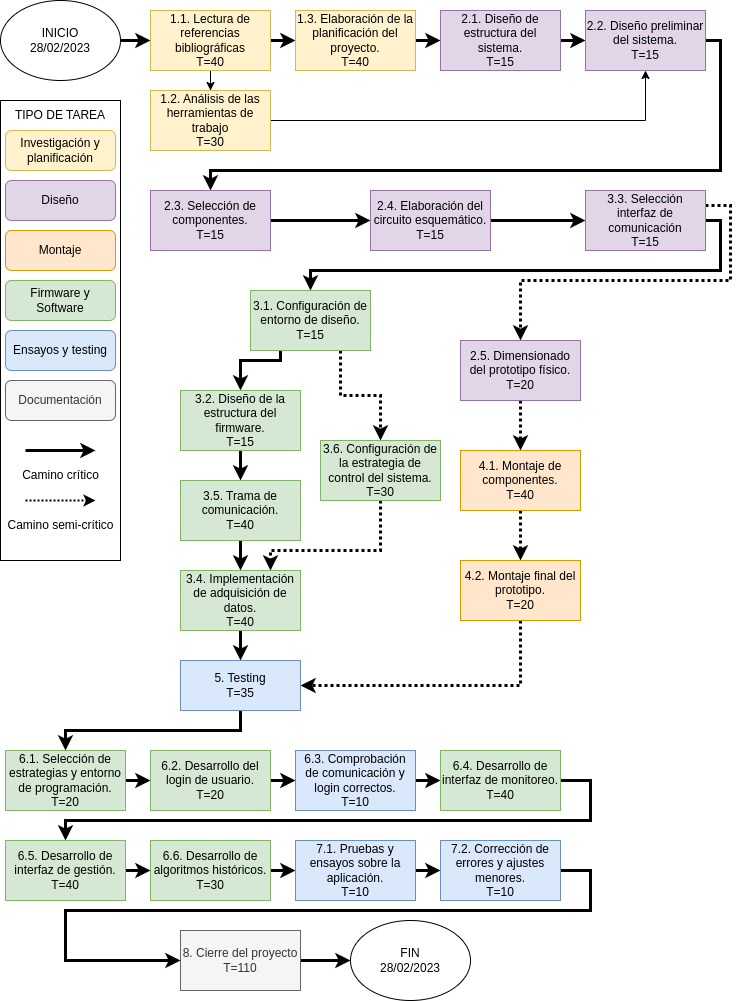
\includegraphics[width=.8\textwidth]{./Figuras/AoN.png}
\caption{Diagrama de \textit{Activity on Node}.}
\label{fig:AoN}
\end{figure}


\section{11. Diagrama de Gantt}
\label{sec:gantt}




\begin{figure}[htpb]
\centering 
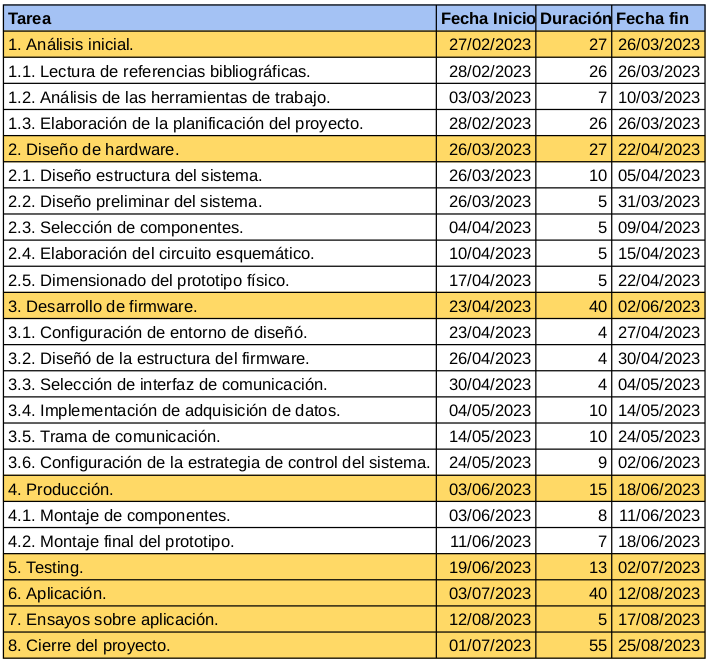
\includegraphics[height=.5\textheight]{./Figuras/TABLA-GANTT.png}
\caption{Diagrama en tabla de WBS}
\label{fig:diagGantt}
\end{figure}

\begin{figure}[htpb]
\centering 
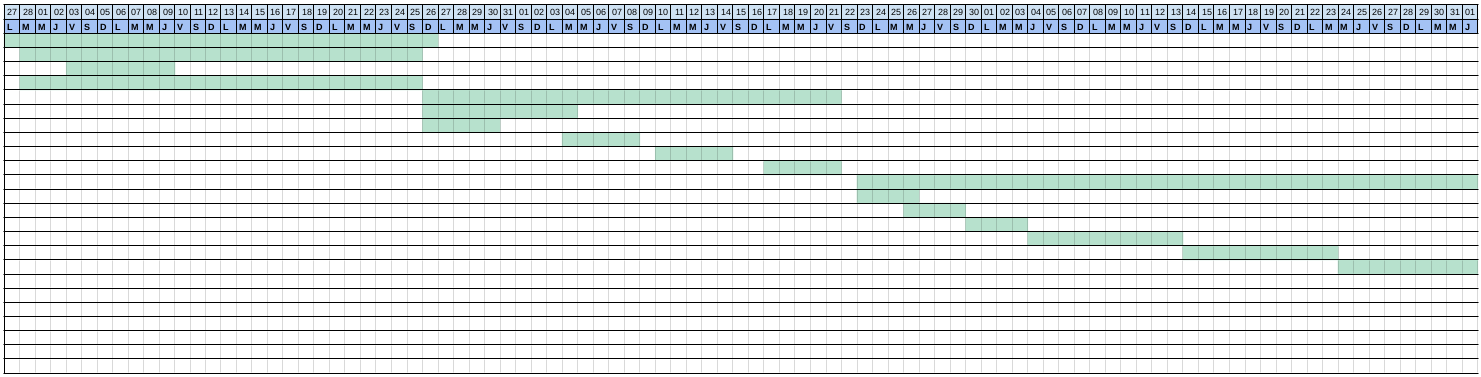
\includegraphics[angle=90, height=.95\textheight]{./Figuras/GANTT-primera.png}
\caption{Primera parte del diagrama de Gantt, inicio del proyecto}
\label{fig:diagGantt}
\end{figure}

\begin{figure}[htpb]
\centering 
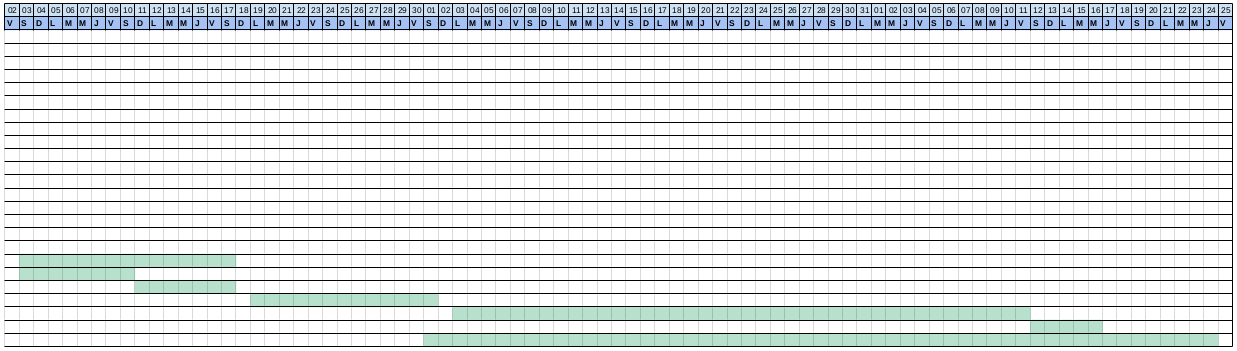
\includegraphics[angle=90, height=.95\textheight]{./Figuras/GANTT-segunda.png}
\caption{Segunda parte del diagrama de Gantt, fin del proyecto}
\label{fig:diagGantt}
\end{figure}



\section{12. Presupuesto detallado del proyecto}
\label{sec:presupuesto}

\begin{consigna}{red}
Si el proyecto es complejo entonces separarlo en partes:
\begin{itemize}
	\item Un total global, indicando el subtotal acumulado por cada una de las áreas.
	\item El desglose detallado del subtotal de cada una de las áreas.
\end{itemize}

IMPORTANTE: No olvidarse de considerar los COSTOS INDIRECTOS.

\end{consigna}

\begin{table}[htpb]
\centering
\begin{tabularx}{\linewidth}{@{}|X|c|r|r|@{}}
\hline
\rowcolor[HTML]{C0C0C0} 
\multicolumn{4}{|c|}{\cellcolor[HTML]{C0C0C0}COSTOS DIRECTOS} \\ \hline
\rowcolor[HTML]{C0C0C0} 
Descripción &
  \multicolumn{1}{c|}{\cellcolor[HTML]{C0C0C0}Cantidad} &
  \multicolumn{1}{c|}{\cellcolor[HTML]{C0C0C0}Valor unitario} &
  \multicolumn{1}{c|}{\cellcolor[HTML]{C0C0C0}Valor total} \\ \hline
 &
  \multicolumn{1}{c|}{} &
  \multicolumn{1}{c|}{} &
  \multicolumn{1}{c|}{} \\ \hline
 &
  \multicolumn{1}{c|}{} &
  \multicolumn{1}{c|}{} &
  \multicolumn{1}{c|}{} \\ \hline
\multicolumn{1}{|l|}{} &
   &
   &
   \\ \hline
\multicolumn{1}{|l|}{} &
   &
   &
   \\ \hline
\multicolumn{3}{|c|}{SUBTOTAL} &
  \multicolumn{1}{c|}{} \\ \hline
\rowcolor[HTML]{C0C0C0} 
\multicolumn{4}{|c|}{\cellcolor[HTML]{C0C0C0}COSTOS INDIRECTOS} \\ \hline
\rowcolor[HTML]{C0C0C0} 
Descripción &
  \multicolumn{1}{c|}{\cellcolor[HTML]{C0C0C0}Cantidad} &
  \multicolumn{1}{c|}{\cellcolor[HTML]{C0C0C0}Valor unitario} &
  \multicolumn{1}{c|}{\cellcolor[HTML]{C0C0C0}Valor total} \\ \hline
\multicolumn{1}{|l|}{} &
   &
   &
   \\ \hline
\multicolumn{1}{|l|}{} &
   &
   &
   \\ \hline
\multicolumn{1}{|l|}{} &
   &
   &
   \\ \hline
\multicolumn{3}{|c|}{SUBTOTAL} &
  \multicolumn{1}{c|}{} \\ \hline
\rowcolor[HTML]{C0C0C0}
\multicolumn{3}{|c|}{TOTAL} &
   \\ \hline
\end{tabularx}%
\end{table}


\section{13. Gestión de riesgos}
\label{sec:riesgos}

\begin{consigna}{red}
a) Identificación de los riesgos (al menos cinco) y estimación de sus consecuencias:
 
Riesgo 1: detallar el riesgo (riesgo es algo que si ocurre altera los planes previstos de forma negativa)
\begin{itemize}
	\item Severidad (S): mientras más severo, más alto es el número (usar números del 1 al 10).\\
	Justificar el motivo por el cual se asigna determinado número de severidad (S).
	\item Probabilidad de ocurrencia (O): mientras más probable, más alto es el número (usar del 1 al 10).\\
	Justificar el motivo por el cual se asigna determinado número de (O). 
\end{itemize}   

Riesgo 2:
\begin{itemize}
	\item Severidad (S): 
	\item Ocurrencia (O):
\end{itemize}

Riesgo 3:
\begin{itemize}
	\item Severidad (S): 
	\item Ocurrencia (O):
\end{itemize}


b) Tabla de gestión de riesgos:      (El RPN se calcula como RPN=SxO)

\begin{table}[htpb]
\centering
\begin{tabularx}{\linewidth}{@{}|X|c|c|c|c|c|c|@{}}
\hline
\rowcolor[HTML]{C0C0C0} 
Riesgo & S & O & RPN & S* & O* & RPN* \\ \hline
       &   &   &     &    &    &      \\ \hline
       &   &   &     &    &    &      \\ \hline
       &   &   &     &    &    &      \\ \hline
       &   &   &     &    &    &      \\ \hline
       &   &   &     &    &    &      \\ \hline
\end{tabularx}%
\end{table}

Criterio adoptado: 
Se tomarán medidas de mitigación en los riesgos cuyos números de RPN sean mayores a...

Nota: los valores marcados con (*) en la tabla corresponden luego de haber aplicado la mitigación.

c) Plan de mitigación de los riesgos que originalmente excedían el RPN máximo establecido:
 
Riesgo 1: plan de mitigación (si por el RPN fuera necesario elaborar un plan de mitigación).
  Nueva asignación de S y O, con su respectiva justificación:
  - Severidad (S): mientras más severo, más alto es el número (usar números del 1 al 10).
          Justificar el motivo por el cual se asigna determinado número de severidad (S).
  - Probabilidad de ocurrencia (O): mientras más probable, más alto es el número (usar del 1 al 10).
          Justificar el motivo por el cual se asigna determinado número de (O).

Riesgo 2: plan de mitigación (si por el RPN fuera necesario elaborar un plan de mitigación).
 
Riesgo 3: plan de mitigación (si por el RPN fuera necesario elaborar un plan de mitigación).

\end{consigna}


\section{14. Gestión de la calidad}
\label{sec:calidad}

\begin{consigna}{red}
Para cada uno de los requerimientos del proyecto indique:
\begin{itemize} 
\item Req \#1: copiar acá el requerimiento.

\begin{itemize}
	\item Verificación para confirmar si se cumplió con lo requerido antes de mostrar el sistema al cliente. Detallar 
	\item Validación con el cliente para confirmar que está de acuerdo en que se cumplió con lo requerido. Detallar  
\end{itemize}

\end{itemize}

Tener en cuenta que en este contexto se pueden mencionar simulaciones, cálculos, revisión de hojas de datos, consulta con expertos, mediciones, etc.  Las acciones de verificación suelen considerar al entregable como ``caja blanca'', es decir se conoce en profundidad su funcionamiento interno.  En cambio, las acciones de validación suelen considerar al entregable como ``caja negra'', es decir, que no se conocen los detalles de su funcionamiento interno.

\end{consigna}

\section{15. Procesos de cierre}    
\label{sec:cierre}

\begin{consigna}{red}
Establecer las pautas de trabajo para realizar una reunión final de evaluación del proyecto, tal que contemple las siguientes actividades:

\begin{itemize}
	\item Pautas de trabajo que se seguirán para analizar si se respetó el Plan de Proyecto original:
	 - Indicar quién se ocupará de hacer esto y cuál será el procedimiento a aplicar. 
	\item Identificación de las técnicas y procedimientos útiles e inútiles que se emplearon, y los problemas que surgieron y cómo se solucionaron:
	 - Indicar quién se ocupará de hacer esto y cuál será el procedimiento para dejar registro.
	\item Indicar quién organizará el acto de agradecimiento a todos los interesados, y en especial al equipo de trabajo y colaboradores:
	  - Indicar esto y quién financiará los gastos correspondientes.
\end{itemize}

\end{consigna}


\end{document}
